% This LaTeX was auto-generated from MATLAB code.
% To make changes, update the MATLAB code and export to LaTeX again.

\documentclass{article}

\usepackage[utf8]{inputenc}  % Allows Unicode characters
\usepackage[T1]{fontenc}     % Ensures correct font encoding
\usepackage{lmodern}         % Modern font
\usepackage{graphicx}        % For images
\usepackage{color}           % For text color
\usepackage{hyperref}        % For hyperlinks
\usepackage{amsmath}         % Math symbols
\usepackage{amsfonts}        % More math symbols
\usepackage{epstopdf}        % EPS to PDF conversion
\usepackage[table]{xcolor}   % For table colors
\usepackage{matlab}          % If this is the correct package (else use matlab-prettifier)
\usepackage[paperheight=795pt,paperwidth=614pt,top=72pt,bottom=72pt,right=72pt,left=72pt,heightrounded]{geometry}
\usepackage[numbered,framed]{matlab-prettifier}  % MATLAB code formatting
\usepackage{textcomp}        % Provides extra symbols

\sloppy
\epstopdfsetup{outdir=./}
\graphicspath{ {./homework_2_media/} }

\begin{document}

\matlabtitle{Homework 2}

\matlabheading{AME 5763}

\matlabheading{Blake Johnson}

\vspace{1em}


\vspace{1em}
\matlabheadingtwo{Problem 4.1: 		}

\matlabheadingtwo{Consider a four node cubic element in one dimension. The element length is 3 with $x_1 =-1$; the remaining nodes are equally spaced. }


\vspace{1em}
\matlabheadingthree{Part A: }

\matlabheadingthree{Construct the Element Shape Function}

\begin{par}
\hfill \break
\end{par}

\begin{matlabcode}
%% Define the shape functions for a 1D cubic element.

syms x

x_1 = -1;
x_2 = 0;
x_3 = 1;
x_4 = 2;
% Shape function N1(x)
N1 = ((x-x_2)*(x-x_3)*(x-x_4))/((x_1-x_2)*(x_1-x_3)*(x_1-x_4));
% Shape function N2(x)
N2 = ((x-x_1)*(x-x_3)*(x-x_4))/((x_2-x_1)*(x_2-x_3)*(x_2-x_4));
% Shape function N3(x)
N3 = ((x-x_1)*(x-x_2)*(x-x_4))/((x_3-x_1)*(x_3-x_2)*(x_3-x_4));
% Shape function N4(x)
N4 = ((x-x_1)*(x-x_2)*(x-x_3))/((x_4-x_1)*(x_4-x_2)*(x_4-x_3));

\end{matlabcode}

\begin{par}
\begin{flushleft}
The Element Shape functions are:
\end{flushleft}
\end{par}

\begin{matlabcode}
disp(N1)
\end{matlabcode}
\begin{matlabsymbolicoutput}
\hskip1em $\displaystyle -\frac{x\,{\left(x-1\right)}\,{\left(x-2\right)}}{6}$
\end{matlabsymbolicoutput}
\begin{matlabcode}
disp(N2)
\end{matlabcode}
\begin{matlabsymbolicoutput}
\hskip1em $\displaystyle \frac{{\left(x-1\right)}\,{\left(x+1\right)}\,{\left(x-2\right)}}{2}$
\end{matlabsymbolicoutput}
\begin{matlabcode}
disp(N3)
\end{matlabcode}
\begin{matlabsymbolicoutput}
\hskip1em $\displaystyle -\frac{x\,{\left(x+1\right)}\,{\left(x-2\right)}}{2}$
\end{matlabsymbolicoutput}
\begin{matlabcode}
disp(N4)
\end{matlabcode}
\begin{matlabsymbolicoutput}
\hskip1em $\displaystyle \frac{x\,{\left(x-1\right)}\,{\left(x+1\right)}}{6}$
\end{matlabsymbolicoutput}
\begin{matlabcode}

\end{matlabcode}

\matlabheadingthree{Part B: }

\matlabheadingthree{Find the displacement field when}

\matlabheadingthree{$$d^e =\left(\begin{array}{c}
u_1 \\
u_2 \\
u_3 \\
u_4 
\end{array}\right)=10^{-3} \left(\begin{array}{c}
1\\
0\\
1\\
4
\end{array}\right)$$}


\vspace{1em}
\begin{matlabcode}

u1 = 1e-3;
u2 = 0;
u3 = 1e-3;
u4 = 4e-3;

u = [u1; u2; u3; u4];
% Displacement field u(x)
u_x = N1*u1 + N2*u2 + N3*u3 + N4*u4;

% Simplify the expression for clarity
u_x_simplified = simplify(u_x);

\end{matlabcode}

\begin{par}
\begin{flushleft}
The displacement field in the element with the given parameters is:
\end{flushleft}
\end{par}

\begin{matlabcode}
disp(u_x)
\end{matlabcode}
\begin{matlabsymbolicoutput}
\hskip1em $\displaystyle \frac{x\,{\left(x-1\right)}\,{\left(x+1\right)}}{1500}-\frac{x\,{\left(x-1\right)}\,{\left(x-2\right)}}{6000}-\frac{x\,{\left(x+1\right)}\,{\left(x-2\right)}}{2000}$
\end{matlabsymbolicoutput}
\begin{matlabcode}
disp(u_x_simplified)
\end{matlabcode}
\begin{matlabsymbolicoutput}
\hskip1em $\displaystyle \frac{x^2 }{1000}$
\end{matlabsymbolicoutput}
\begin{matlabcode}

\end{matlabcode}

\matlabheadingthree{Part C: }

\matlabheadingthree{Evaluate the $B^e$ matrix and find the strain for the above displacement field.}

\begin{par}
\hfill \break
\end{par}

\begin{matlabcode}
% The B matrix is the matirx that relates the nodal displacement to the
% strain of the element

e_1 = diff(N1,x);
e_2 = diff(N2,x);
e_3 = diff(N3,x);
e_4 = diff(N4,x);

B_e = [e_1 e_2 e_3 e_4];

% Strain of the displacement field is B_e*u(x)

strain = B_e * u;
strain_simplify = simplify(strain);
\end{matlabcode}

\begin{par}
\begin{flushleft}
The strain for the displacement field is:
\end{flushleft}
\end{par}

\begin{matlabcode}
disp(strain)
\end{matlabcode}
\begin{matlabsymbolicoutput}
\hskip1em $\displaystyle \frac{{\left(x-1\right)}\,{\left(x+1\right)}}{1500}-\frac{{\left(x-1\right)}\,{\left(x-2\right)}}{6000}-\frac{{\left(x+1\right)}\,{\left(x-2\right)}}{2000}+\frac{x\,{\left(x-1\right)}}{2000}+\frac{x\,{\left(x+1\right)}}{6000}-\frac{x\,{\left(x-2\right)}}{1500}$
\end{matlabsymbolicoutput}
\begin{matlabcode}
disp(strain_simplify)
\end{matlabcode}
\begin{matlabsymbolicoutput}
\hskip1em $\displaystyle \frac{x}{500}$
\end{matlabsymbolicoutput}

\matlabheadingthree{Part D: }

\matlabheadingthree{Plot the Displacement Field $u(x)$ and Strain Field $\epsilon (x)$}


\vspace{1em}
\begin{matlabcode}
% Define a range for x from -1 to 2 (element length)
x_vals = linspace(-1, 2, 100);

% Convert symbolic expressions to MATLAB functions for plotting
u_x_func = matlabFunction(u_x_simplified);
strain_x_func = matlabFunction(strain_simplify);

% Compute displacement and strain values over the range of x
u_vals = u_x_func(x_vals);
strain_vals = strain_x_func(x_vals);

\end{matlabcode}

\begin{par}
\begin{flushleft}
Plots of the displacement u(x) and the strain e(x):
\end{flushleft}
\end{par}

\begin{matlabcode}
% Plot displacement field alone
figure;
plot(x_vals, u_vals, 'LineWidth', 2);
title('Displacement Field u(x)');
xlabel('x');
ylabel('Displacement u(x)');
grid on;
\end{matlabcode}
\begin{center}
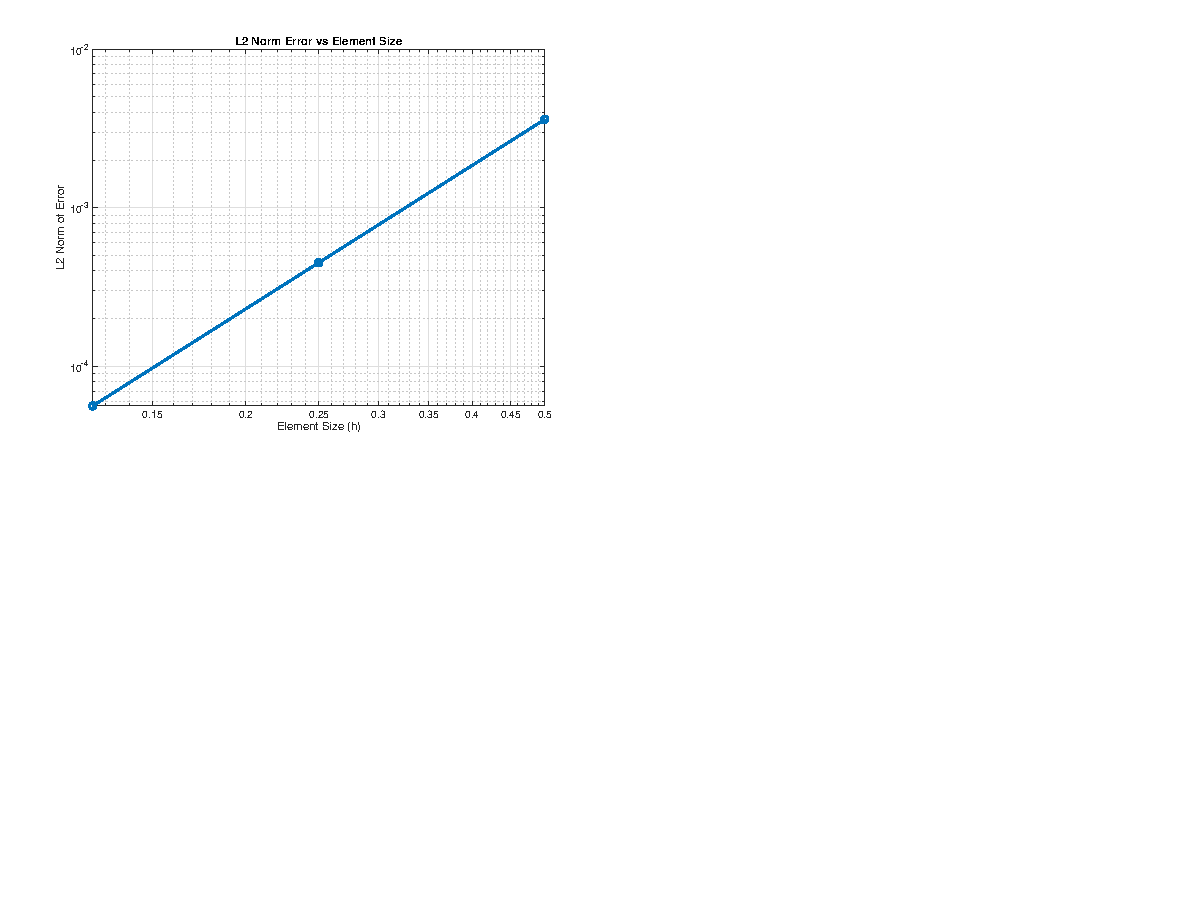
\includegraphics[width=\maxwidth{56.196688409433015em}]{figure_0.eps}
\end{center}
\begin{matlabcode}

% Plot strain field alone
figure;
plot(x_vals, strain_vals, 'LineWidth', 2, 'Color', 'r');
title('Strain Field \epsilon(x)');
xlabel('x');
ylabel('Strain \epsilon(x)');
grid on;
\end{matlabcode}
\begin{center}
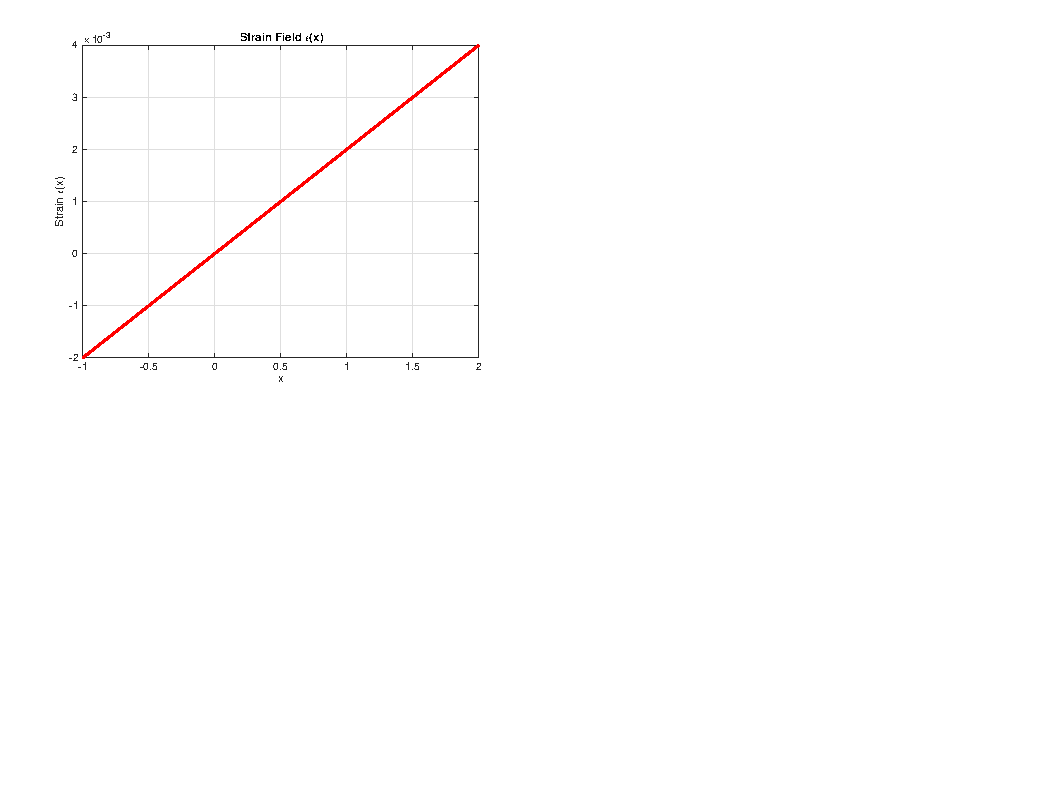
\includegraphics[width=\maxwidth{56.196688409433015em}]{figure_1.eps}
\end{center}

\matlabheadingthree{Part E: }

\matlabheadingthree{Find the Strain Field when the nodal displacements are $d^{eT} =[1111]$. Why is the result expected?}

\begin{par}
\hfill \break
\end{par}

\begin{matlabcode}
% Nodal displacements d^e = [1 1 1 1]
u1_new = 1;
u2_new = 1;
u3_new = 1;
u4_new = 1;

% New displacement field u(x)
u_new = N1*u1_new + N2*u2_new + N3*u3_new + N4*u4_new;

% New strain field (derivative of u(x))
strain_new = diff(u_new, x);

% Simplify the new strain expression
strain_new_simplified = simplify(strain_new);

% Display the new strain (which should be zero)
\end{matlabcode}

\begin{par}
\begin{flushleft}
The new strain field with uniform nodal displacement is:
\end{flushleft}
\end{par}

\begin{matlabcode}
disp(strain_x_new_simplified);
\end{matlabcode}
\begin{matlabsymbolicoutput}
\hskip1em $\displaystyle 0$
\end{matlabsymbolicoutput}

\begin{par}
\begin{flushleft}
This is expected because the all the nodes have the same displacement. So the bar is moving the same distane and the length of the bar does not change.
\end{flushleft}
\end{par}



\vspace{1em}

\vspace{1em}
\matlabheadingtwo{4.3:				}

\matlabheadingtwo{Derive the shape functions for a two-node one-dimensional element which is $C^1$ continuous. Note that the shape functions derived in Chapter 4 are $C^0$ continuous. To enforce $C^1$ continuity, it is necessary to enforce continuity of displacements and their derivatives. Start by considering a complete cubic approximation $u^e =\alpha_0^e +\alpha_1^e x+\alpha_2^e x^2 +\alpha_3^e x^3$ and derive four shape functions corresponding to the displacements and their derivatives at each node. }

\begin{matlabcode}
syms y

M = [1 x x^2 x^3; 0 1 2*x 3*x^2; 1 y y^2 y^3; 0 1 2*y 3*y^2];

M_i = inv(M)
\end{matlabcode}
\begin{matlabsymbolicoutput}
M\_i = 

\hskip1em $\displaystyle \begin{array}{l}
\left(\begin{array}{cccc}
\frac{\sigma_6 -y^3 }{\sigma_4 } & -\frac{x\,y^2 }{\sigma_1 } & -\frac{\sigma_5 -x^3 }{\sigma_4 } & -\frac{x^2 \,y}{\sigma_1 }\\
-\sigma_3  & \frac{y^2 +2\,x\,y}{\sigma_1 } & \sigma_3  & \frac{x^2 +2\,y\,x}{\sigma_1 }\\
\sigma_2  & -\frac{x+2\,y}{\sigma_1 } & -\sigma_2  & -\frac{2\,x+y}{\sigma_1 }\\
-\frac{2}{\sigma_4 } & \frac{1}{\sigma_1 } & \frac{2}{\sigma_4 } & \frac{1}{\sigma_1 }
\end{array}\right)\\
\mathrm{}\\
\textrm{where}\\
\mathrm{}\\
\;\;\sigma_1 =x^2 -2\,x\,y+y^2 \\
\mathrm{}\\
\;\;\sigma_2 =\frac{3\,{\left(x+y\right)}}{\sigma_4 }\\
\mathrm{}\\
\;\;\sigma_3 =\frac{6\,x\,y}{\sigma_4 }\\
\mathrm{}\\
\;\;\sigma_4 =x^3 -\sigma_5 +\sigma_6 -y^3 \\
\mathrm{}\\
\;\;\sigma_5 =3\,x^2 \,y\\
\mathrm{}\\
\;\;\sigma_6 =3\,x\,y^2 
\end{array}$
\end{matlabsymbolicoutput}
\begin{matlabcode}
p1 = M(1,:);

p2 = M(2,:);

p3 = M(3,:);

p4 = M(4,:);

N1 = p1 * M_i;

N2 = p2 * M_i;
N3 = p3 * M_i;

N4 = p4 * M_i;


disp(N1);
\end{matlabcode}
\begin{matlabsymbolicoutput}
\hskip1em $\displaystyle \begin{array}{l}
\left(\begin{array}{cccc}
\frac{\sigma_7 -y^3 }{\sigma_5 }-\sigma_4 +\sigma_2 -\sigma_3  & \frac{x^3 }{\sigma_1 }+\frac{x\,{\left(y^2 +2\,x\,y\right)}}{\sigma_1 }-\frac{x\,y^2 }{\sigma_1 }-\frac{x^2 \,{\left(x+2\,y\right)}}{\sigma_1 } & \sigma_4 -\frac{\sigma_6 -x^3 }{\sigma_5 }-\sigma_2 +\sigma_3  & \frac{x^3 }{\sigma_1 }+\frac{x\,{\left(x^2 +2\,y\,x\right)}}{\sigma_1 }-\frac{x^2 \,y}{\sigma_1 }-\frac{x^2 \,{\left(2\,x+y\right)}}{\sigma_1 }
\end{array}\right)\\
\mathrm{}\\
\textrm{where}\\
\mathrm{}\\
\;\;\sigma_1 =x^2 -2\,x\,y+y^2 \\
\mathrm{}\\
\;\;\sigma_2 =\frac{3\,x^2 \,{\left(x+y\right)}}{\sigma_5 }\\
\mathrm{}\\
\;\;\sigma_3 =\frac{6\,x^2 \,y}{\sigma_5 }\\
\mathrm{}\\
\;\;\sigma_4 =\frac{2\,x^3 }{\sigma_5 }\\
\mathrm{}\\
\;\;\sigma_5 =x^3 -\sigma_6 +\sigma_7 -y^3 \\
\mathrm{}\\
\;\;\sigma_6 =3\,x^2 \,y\\
\mathrm{}\\
\;\;\sigma_7 =3\,x\,y^2 
\end{array}$
\end{matlabsymbolicoutput}
\begin{matlabcode}

disp(N2);
\end{matlabcode}
\begin{matlabsymbolicoutput}
\hskip1em $\displaystyle \begin{array}{l}
\left(\begin{array}{cccc}
\sigma_1 -\sigma_2 -\frac{6\,x\,y}{\sigma_4 } & \frac{y^2 +2\,x\,y}{\sigma_5 }+\sigma_3 -\frac{2\,x\,{\left(x+2\,y\right)}}{\sigma_5 } & \sigma_2 -\sigma_1 +\frac{6\,x\,y}{\sigma_4 } & \frac{x^2 +2\,y\,x}{\sigma_5 }+\sigma_3 -\frac{2\,x\,{\left(2\,x+y\right)}}{\sigma_5 }
\end{array}\right)\\
\mathrm{}\\
\textrm{where}\\
\mathrm{}\\
\;\;\sigma_1 =\frac{6\,x\,{\left(x+y\right)}}{\sigma_4 }\\
\mathrm{}\\
\;\;\sigma_2 =\frac{6\,x^2 }{\sigma_4 }\\
\mathrm{}\\
\;\;\sigma_3 =\frac{3\,x^2 }{\sigma_5 }\\
\mathrm{}\\
\;\;\sigma_4 =x^3 -3\,x^2 \,y+3\,x\,y^2 -y^3 \\
\mathrm{}\\
\;\;\sigma_5 =x^2 -2\,x\,y+y^2 
\end{array}$
\end{matlabsymbolicoutput}
\begin{matlabcode}

disp(N3);
\end{matlabcode}
\begin{matlabsymbolicoutput}
\hskip1em $\displaystyle \begin{array}{l}
\left(\begin{array}{cccc}
\frac{\sigma_7 -y^3 }{\sigma_5 }-\sigma_4 +\sigma_2 -\sigma_3  & \frac{y^3 }{\sigma_1 }+\frac{y\,{\left(y^2 +2\,x\,y\right)}}{\sigma_1 }-\frac{x\,y^2 }{\sigma_1 }-\frac{y^2 \,{\left(x+2\,y\right)}}{\sigma_1 } & \sigma_4 -\frac{\sigma_6 -x^3 }{\sigma_5 }-\sigma_2 +\sigma_3  & \frac{y^3 }{\sigma_1 }+\frac{y\,{\left(x^2 +2\,y\,x\right)}}{\sigma_1 }-\frac{x^2 \,y}{\sigma_1 }-\frac{y^2 \,{\left(2\,x+y\right)}}{\sigma_1 }
\end{array}\right)\\
\mathrm{}\\
\textrm{where}\\
\mathrm{}\\
\;\;\sigma_1 =x^2 -2\,x\,y+y^2 \\
\mathrm{}\\
\;\;\sigma_2 =\frac{3\,y^2 \,{\left(x+y\right)}}{\sigma_5 }\\
\mathrm{}\\
\;\;\sigma_3 =\frac{6\,x\,y^2 }{\sigma_5 }\\
\mathrm{}\\
\;\;\sigma_4 =\frac{2\,y^3 }{\sigma_5 }\\
\mathrm{}\\
\;\;\sigma_5 =x^3 -\sigma_6 +\sigma_7 -y^3 \\
\mathrm{}\\
\;\;\sigma_6 =3\,x^2 \,y\\
\mathrm{}\\
\;\;\sigma_7 =3\,x\,y^2 
\end{array}$
\end{matlabsymbolicoutput}
\begin{matlabcode}

disp(N4);
\end{matlabcode}
\begin{matlabsymbolicoutput}
\hskip1em $\displaystyle \begin{array}{l}
\left(\begin{array}{cccc}
\sigma_1 -\sigma_2 -\frac{6\,x\,y}{\sigma_4 } & \frac{y^2 +2\,x\,y}{\sigma_5 }+\sigma_3 -\frac{2\,y\,{\left(x+2\,y\right)}}{\sigma_5 } & \sigma_2 -\sigma_1 +\frac{6\,x\,y}{\sigma_4 } & \frac{x^2 +2\,y\,x}{\sigma_5 }+\sigma_3 -\frac{2\,y\,{\left(2\,x+y\right)}}{\sigma_5 }
\end{array}\right)\\
\mathrm{}\\
\textrm{where}\\
\mathrm{}\\
\;\;\sigma_1 =\frac{6\,y\,{\left(x+y\right)}}{\sigma_4 }\\
\mathrm{}\\
\;\;\sigma_2 =\frac{6\,y^2 }{\sigma_4 }\\
\mathrm{}\\
\;\;\sigma_3 =\frac{3\,y^2 }{\sigma_5 }\\
\mathrm{}\\
\;\;\sigma_4 =x^3 -3\,x^2 \,y+3\,x\,y^2 -y^3 \\
\mathrm{}\\
\;\;\sigma_5 =x^2 -2\,x\,y+y^2 
\end{array}$
\end{matlabsymbolicoutput}



\vspace{1em}
\matlabheadingtwo{4.4:}

\matlabheadingtwo{Consider the displacement field u(x) = $x^3 ,0\le x\le 1$. Write a MATLAB program that performs the following tasks:}


\vspace{1em}
\matlabheadingthree{Part A: }

\matlabheadingthree{Subdivide the interval [0,1] into two elements. Compute the displacement field in each element by letting the nodal displacements be given by $u_1 =x_1^3$ and using a linear two-node element so that the displacement field in each element is given by $u^e (x)={{\textrm{N}}}^{{\textrm{e}}} (x){{\textrm{d}}}^{{\textrm{e}}} ={{\textrm{N}}}^{{\textrm{e}}} (x){{\textrm{L}}}^{{\textrm{e}}} {\textrm{d}}$, where ${{\textrm{N}}}^{{\textrm{e}}} (x)$ are the linear shae functions given by (4.6). Plot $u(x)$ and the finite element field $u^e (x)$ on the smae plot in the interval [0,1].}

\begin{par}
\hfill \break
\end{par}

\begin{matlabcode}
% Set up the length of the interval and divide evenly so the two elements
% are symmetrical
x1 = 0;
x3 = 1;
x2 = (x1 + x3)/2;  % Midpoint

% Nodal displacements (cubic function u(x) = x^3)
u_11 = (x1)^3;  % u at node 1 for element 1
u_12 = (x2)^3;  % u at node 2 for element 1
u_21 = (x2)^3;  % u at node 1 for element 2
u_22 = (x3)^3;  % u at node 2 for element 2

% Shape functions for Element 1 (from x1 to x2)
syms x
N_11 = (x - x2) / (x1 - x2);
N_12 = (x - x1) / (x2 - x1);

% Displacement field for Element 1
u_1 = N_11 * u_11 + N_12 * u_12;

% Shape functions for Element 2 (from x2 to x3)
N_21 = (x3 - x) / (x3 - x2);
N_22 = (x - x2) / (x3 - x2);

% Displacement field for Element 2
u_2 = N_21 * u_21 + N_22 * u_22;

% Check boundary conditions
u_11  % Should be 0 at node 1 of element 1
\end{matlabcode}
\begin{matlaboutput}
u_11 =      0
\end{matlaboutput}
\begin{matlabcode}
u_12  % Should match u_21 to ensure continuity between elements
\end{matlabcode}
\begin{matlaboutput}
u_12 =    0.125000000000000
\end{matlaboutput}
\begin{matlabcode}
u_21  % Should match u_12
\end{matlabcode}
\begin{matlaboutput}
u_21 =    0.125000000000000
\end{matlaboutput}
\begin{matlabcode}
u_22  % Should be 1 at node 2 of element 2
\end{matlabcode}
\begin{matlaboutput}
u_22 =      1
\end{matlaboutput}
\begin{matlabcode}

% Define the range of x values for each element
x_vals_element1 = linspace(0, 0.5, 100);  % For Element 1
x_vals_element2 = linspace(0.5, 1, 100);  % For Element 2
x_vals_exact = linspace(0, 1, 200);       % For the exact solution over the whole domain

% Evaluate displacement fields at the specified x values
u_1_vals = double(subs(u_1, x, x_vals_element1));  % Displacement for element 1
u_2_vals = double(subs(u_2, x, x_vals_element2));  % Displacement for element 2

% Exact displacement field: u(x) = x^3
u_exact_vals = x_vals_exact .^ 3;

% Plot the displacement fields
figure;
hold on;  % Allow multiple plots on the same figure

% Plot Element 1
plot(x_vals_element1, u_1_vals, 'r', 'LineWidth', 2, 'DisplayName', 'Element 1 (Linear)');
% Plot Element 2
plot(x_vals_element2, u_2_vals, 'b', 'LineWidth', 2, 'DisplayName', 'Element 2 (Linear)');
% Plot the exact displacement field
plot(x_vals_exact, u_exact_vals, 'k--', 'LineWidth', 2, 'DisplayName', 'Exact (x^3)');

% Add labels and title
xlabel('x');
ylabel('Displacement u(x)');
title('Displacement Fields for Finite Elements and Exact Solution');
legend show;  % Show legend
grid on;
hold off;
\end{matlabcode}
\begin{center}
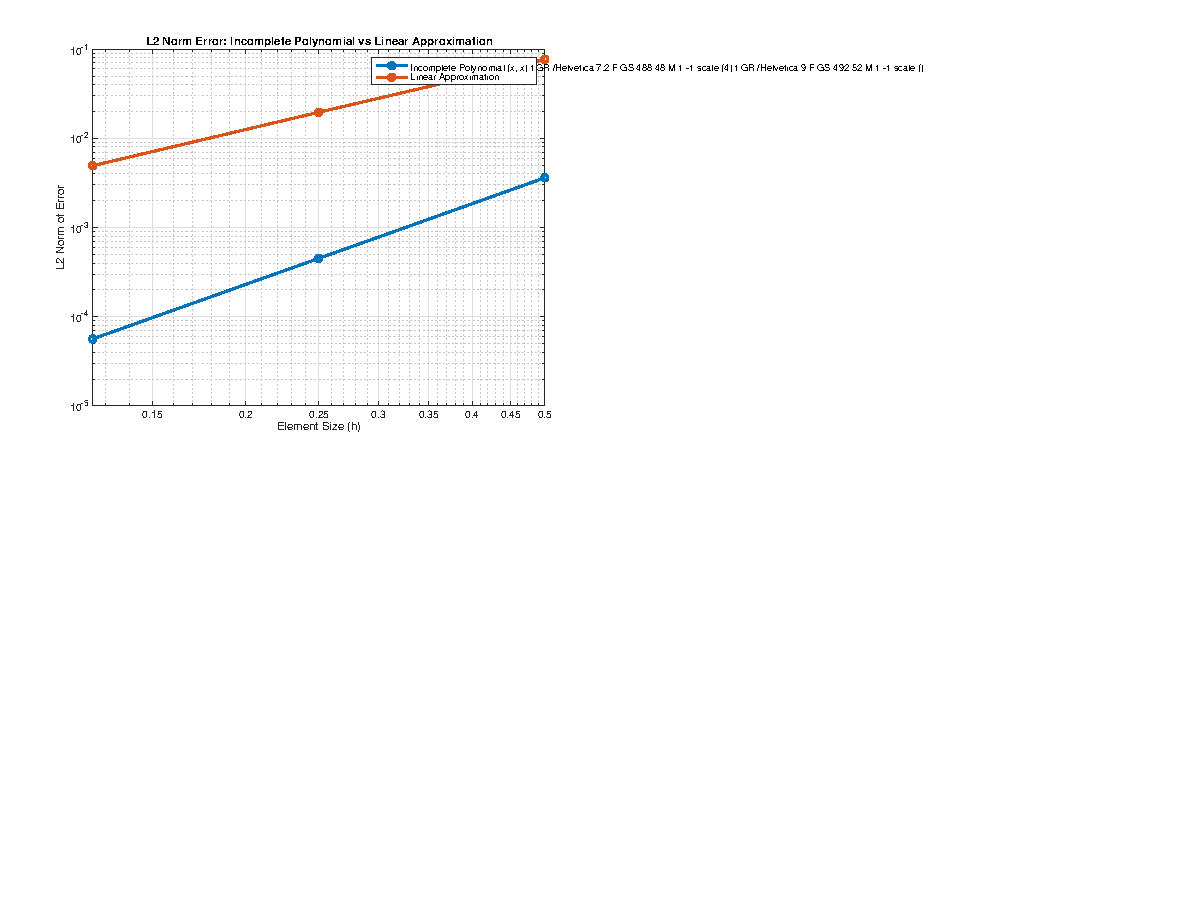
\includegraphics[width=\maxwidth{56.196688409433015em}]{figure_2.eps}
\end{center}

\matlabheadingthree{Part B:}

\matlabheadingthree{Compute the strain in each element by "e ðxÞ 1⁄4 Be ðxÞde 1⁄4 Be ðxÞLe d and plot the finite element strain and the exact strain. How do these compare? }

\begin{par}
\hfill \break
\end{par}

\begin{matlabcode}
% Compute B^e for elements 1 and 2
B_1 = 2*[-1 1];
B_2 = 2*[-1 1];

% Set up a matrix for the displacement vector
d_1 = [u_11 ; u_12];
d_2 = [u_21 ; u_22];

% Strain displacement for element 1 and element 2

e_1 = B_1 * d_1
\end{matlabcode}
\begin{matlaboutput}
e_1 =    0.250000000000000
\end{matlaboutput}
\begin{matlabcode}
e_2 = B_2 * d_2
\end{matlabcode}
\begin{matlaboutput}
e_2 =    1.750000000000000
\end{matlaboutput}
\begin{matlabcode}

% Define the strain for each element (constant within each element)
strain_element1 = 0.25;  % Strain in element 1
strain_element2 = 1.75;  % Strain in element 2

% Define the range of x values for each element
x_vals_element1 = linspace(0, 0.5, 100);  % For Element 1
x_vals_element2 = linspace(0.5, 1, 100);  % For Element 2
x_vals_exact = linspace(0, 1, 200);       % For the exact solution over the whole domain

% Exact strain: e(x) = 3x^2
exact_strain = 3 * x_vals_exact .^ 2;

% Plot the strain fields
figure;
hold on;  % Allow multiple plots on the same figure

% Plot Element 1 strain (constant)
plot(x_vals_element1, strain_element1 * ones(size(x_vals_element1)), 'r', 'LineWidth', 2, 'DisplayName', 'Element 1 Strain (Linear)');
% Plot Element 2 strain (constant)
plot(x_vals_element2, strain_element2 * ones(size(x_vals_element2)), 'b', 'LineWidth', 2, 'DisplayName', 'Element 2 Strain (Linear)');
% Plot the exact strain
plot(x_vals_exact, exact_strain, 'k--', 'LineWidth', 2, 'DisplayName', 'Exact Strain (3x^2)');

% Add labels and title
xlabel('x');
ylabel('Strain \epsilon(x)');
title('Finite Element Strain vs Exact Strain');
legend show;  % Show legend
grid on;
hold off;
\end{matlabcode}
\begin{center}
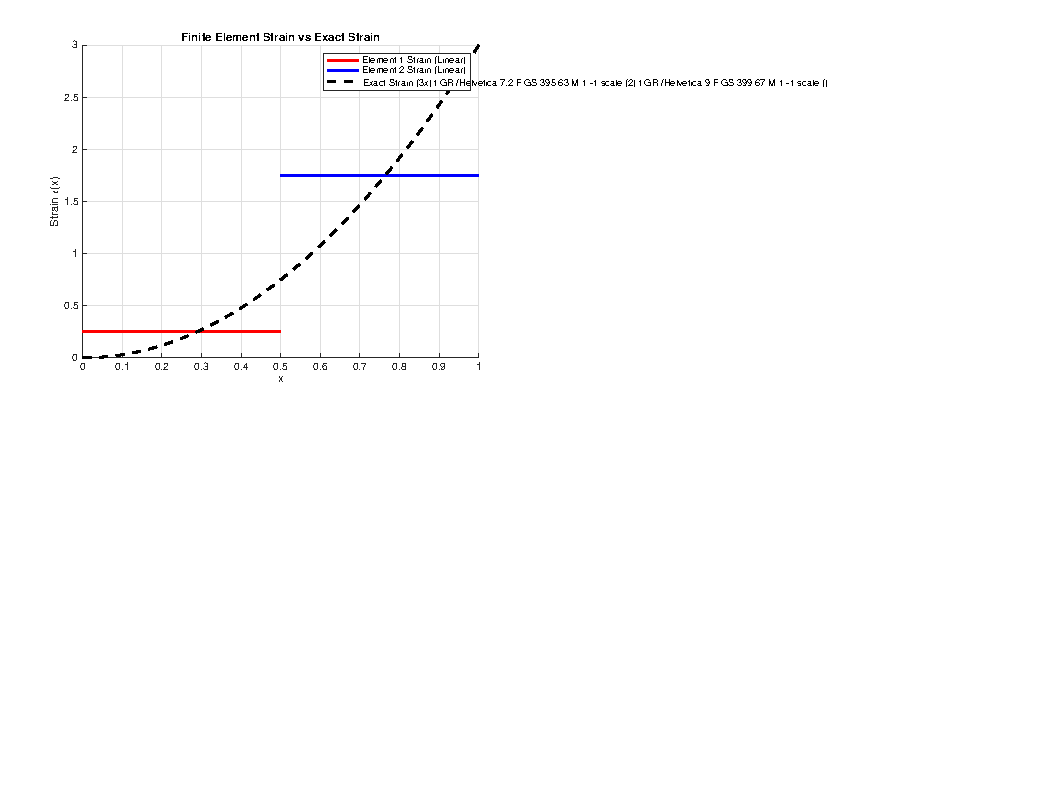
\includegraphics[width=\maxwidth{56.196688409433015em}]{figure_3.eps}
\end{center}

\begin{par}
\begin{flushleft}
The strain on the two elements are constant. Which would be expected since the displacement fields that we used are linear equaitons. The derivatives, ie the strain, of a linear equation would then be constant. However the strain of the actual displacement field is quadratic since the field was a cubic function. So the strain is not a very good approximate, but the values are about what I would expect.
\end{flushleft}
\end{par}


\vspace{1em}
\begin{par}
\begin{flushleft}
		
\end{flushleft}
\end{par}

\begin{par}
\begin{flushleft}
			
\end{flushleft}
\end{par}

\begin{par}
\begin{flushleft}
				
\end{flushleft}
\end{par}

\begin{par}
\begin{flushleft}
											
\end{flushleft}
\end{par}

\matlabheadingthree{Part C:}

\matlabheadingthree{Repeat parts (a) and (b) for meshes of four and eight elements. Does the interpolation of the strain improve? }

\matlabheadingthree{Four Elements}

\begin{par}
\hfill \break
\end{par}

\begin{matlabcode}
% Nodes (using global nodal identifications)
x1 = 0;
x2 = 1/4;
x3 = 1/2;
x4 = 3/4;
x5 = 1;

% Nodal displacements (cubic function u(x) = x^3)

% Element 1
u_11 = (x1)^3;  % u at node 1 for element 1
u_12 = (x2)^3;  % u at node 2 for element 1

% Shape functions for Element 1 (from x1 to x2)
N_11 = (x - x2) / (x1 - x2);
N_12 = (x - x1) / (x2 - x1);

% Displacement field for Element 1
u_1 = N_11 * u_11 + N_12 * u_12;

% Element 2
u_21 = (x2)^3;  % u at node 1 for element 2
u_22 = (x3)^3;  % u at node 2 for element 2

% Shape functions for Element 2 (from x2 to x3)
N_21 = (x3 - x) / (x3 - x2);
N_22 = (x - x2) / (x3 - x2);

% Displacement field for Element 2
u_2 = N_21 * u_21 + N_22 * u_22;

% Element 3
u_31 = (x3)^3;
u_32 = (x4)^3;

% Shape functions for Element 3 (from x2 to x3)
N_31 = (x - x4) / (x3 - x4);
N_32 = (x - x3) / (x4 - x3);

% Displacement field for Element 3
u_3 = N_31 * u_31 + N_32 * u_32;

% Element 4
u_41 = (x4)^3;
u_42 = (x5)^3;

% Shape functions for Element 4 (from x2 to x3)
N_41 = (x - x5) / (x4 - x5);
N_42 = (x - x4) / (x5 - x4);

% Displacement field for Element 4
u_4 = N_41 * u_41 + N_42 * u_42;

% Check boundary conditions
disp(u_11)  % Should be 0 at node 1 of element 1
\end{matlabcode}
\begin{matlaboutput}
     0
\end{matlaboutput}
\begin{matlabcode}
fprintf('u_12 = %.3f, u_21 = %.3f  %% Should be equal\n', u_12, u_21);
\end{matlabcode}
\begin{matlaboutput}
u_12 = 0.016, u_21 = 0.016  % Should be equal
\end{matlaboutput}
\begin{matlabcode}
fprintf('u_22 = %.3f, u_31 = %.3f  %% Should be equal\n', u_22, u_31);
\end{matlabcode}
\begin{matlaboutput}
u_22 = 0.125, u_31 = 0.125  % Should be equal
\end{matlaboutput}
\begin{matlabcode}
fprintf('u_32 = %.3f, u_41 = %.3f  %% Should be equal\n', u_32, u_41);
\end{matlabcode}
\begin{matlaboutput}
u_32 = 0.422, u_41 = 0.422  % Should be equal
\end{matlaboutput}
\begin{matlabcode}
disp(u_42) % Should be 1 at node 2 of element 2
\end{matlabcode}
\begin{matlaboutput}
     1
\end{matlaboutput}
\begin{matlabcode}

% Define the range of x values for each element
x_vals_element1 = linspace(x1, x2, 100);  % For Element 1
x_vals_element2 = linspace(x2, x3, 100);  % For Element 2
x_vals_element3 = linspace(x3, x4, 100);  % For Element 3
x_vals_element4 = linspace(x4, x5, 100);  % For Element 4
x_vals_exact = linspace(x1, x5, 200);     % For the exact solution over the whole domain

% Evaluate displacement fields at the specified x values
u_1_vals = double(subs(u_1, x, x_vals_element1));  % Displacement for Element 1
u_2_vals = double(subs(u_2, x, x_vals_element2));  % Displacement for Element 2
u_3_vals = double(subs(u_3, x, x_vals_element3));  % Displacement for Element 3
u_4_vals = double(subs(u_4, x, x_vals_element4));  % Displacement for Element 4

% Exact displacement field: u(x) = x^3
u_exact_vals = x_vals_exact .^ 3;

% Plot the displacement fields
figure;
hold on;  % Allow multiple plots on the same figure

% Plot Element 1
plot(x_vals_element1, u_1_vals, 'r', 'LineWidth', 2, 'DisplayName', 'Element 1');
% Plot Element 2
plot(x_vals_element2, u_2_vals, 'b', 'LineWidth', 2, 'DisplayName', 'Element 2');
% Plot Element 3
plot(x_vals_element3, u_3_vals, 'g', 'LineWidth', 2, 'DisplayName', 'Element 3');
% Plot Element 4
plot(x_vals_element4, u_4_vals, 'm', 'LineWidth', 2, 'DisplayName', 'Element 4');
% Plot the exact displacement field
plot(x_vals_exact, u_exact_vals, 'k--', 'LineWidth', 2, 'DisplayName', 'Exact (x^3)');

% Add labels and title
xlabel('x');
ylabel('Displacement u(x)');
title('Displacement Fields for Four Elements and Exact Solution');
legend show;  % Show legend
grid on;
hold off;
\end{matlabcode}
\begin{center}
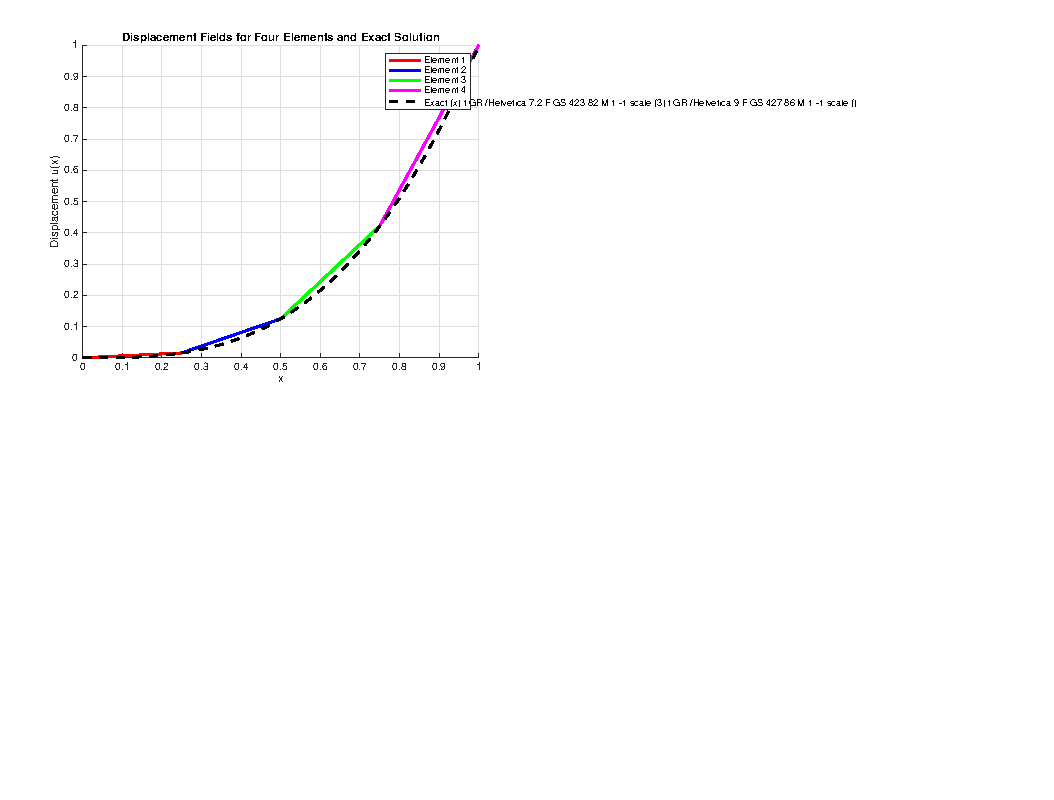
\includegraphics[width=\maxwidth{56.196688409433015em}]{figure_4.eps}
\end{center}

\begin{par}
\begin{flushleft}
			
\end{flushleft}
\end{par}

\begin{matlabcode}
% Compute B^e for all elements
B_1 = 4*[-1 1];
B_2 = 4*[-1 1];
B_3 = 4*[-1 1];
B_4 = 4*[-1 1];

% Set up a matrix for the displacement vector
d_1 = [u_11 ; u_12];
d_2 = [u_21 ; u_22];
d_3 = [u_31 ; u_32];
d_4 = [u_41 ; u_42];

% Strain displacement for element 1 and element 2

e_1 = B_1 * d_1;
e_2 = B_2 * d_2;
e_3 = B_3 * d_3;
e_4 = B_4 * d_4;

% Display computed strains for all elements
disp(e_1);
\end{matlabcode}
\begin{matlaboutput}
   0.062500000000000
\end{matlaboutput}
\begin{matlabcode}
disp(e_2);
\end{matlabcode}
\begin{matlaboutput}
   0.437500000000000
\end{matlaboutput}
\begin{matlabcode}
disp(e_3);
\end{matlabcode}
\begin{matlaboutput}
   1.187500000000000
\end{matlaboutput}
\begin{matlabcode}
disp(e_4);
\end{matlabcode}
\begin{matlaboutput}
   2.312500000000000
\end{matlaboutput}
\begin{matlabcode}

% Define the range of x values for each element (renaming to avoid overwriting previous variables)
x_vals_strain_element1 = linspace(x1, x2, 100);  % For Element 1
x_vals_strain_element2 = linspace(x2, x3, 100);  % For Element 2
x_vals_strain_element3 = linspace(x3, x4, 100);  % For Element 3
x_vals_strain_element4 = linspace(x4, x5, 100);  % For Element 4
x_vals_exact_strain = linspace(x1, x5, 200);     % For the exact solution over the whole domain


% Define the strain for each element (constant within each element)
strain_element1 = e_1(1);  % Strain in element 1
strain_element2 = e_2(1);  % Strain in element 2
strain_element3 = e_3(1);  % Strain in element 3
strain_element4 = e_4(1);  % Strain in element 4

% Plot the strain fields
figure;
hold on;  % Allow multiple plots on the same figure

% Plot Element 1 strain (constant)
plot(x_vals_strain_element1, strain_element1 * ones(size(x_vals_strain_element1)), 'r', 'LineWidth', 2, 'DisplayName', 'Element 1 Strain');
% Plot Element 2 strain (constant)
plot(x_vals_strain_element2, strain_element2 * ones(size(x_vals_strain_element2)), 'b', 'LineWidth', 2, 'DisplayName', 'Element 2 Strain');
% Plot Element 3 strain (constant)
plot(x_vals_strain_element3, strain_element3 * ones(size(x_vals_strain_element3)), 'g', 'LineWidth', 2, 'DisplayName', 'Element 3 Strain');
% Plot Element 4 strain (constant)
plot(x_vals_strain_element4, strain_element4 * ones(size(x_vals_strain_element4)), 'm', 'LineWidth', 2, 'DisplayName', 'Element 4 Strain');
% Plot the exact strain
plot(x_vals_exact_strain, exact_strain, 'k--', 'LineWidth', 2, 'DisplayName', 'Exact Strain (3x^2)');

% Add labels and title
xlabel('x');
ylabel('Strain \epsilon(x)');
title('Finite Element Strain vs Exact Strain');
legend show;  % Show legend
grid on;
hold off;
\end{matlabcode}
\begin{center}
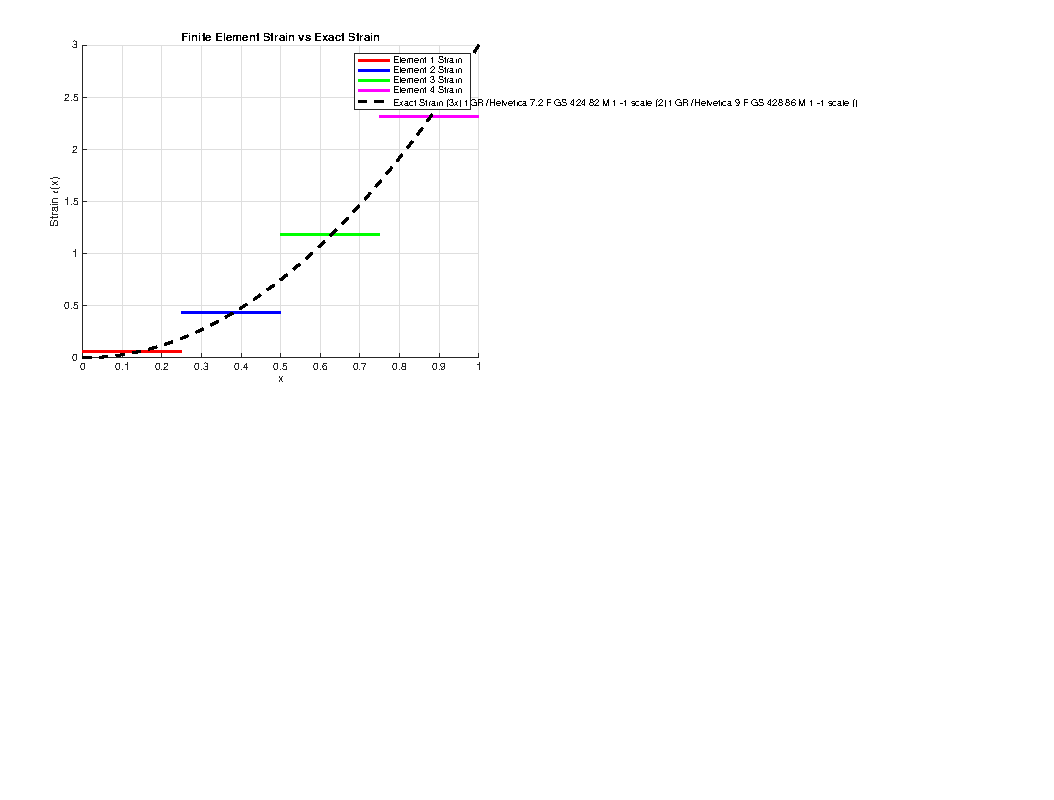
\includegraphics[width=\maxwidth{56.196688409433015em}]{figure_5.eps}
\end{center}

\begin{par}
\begin{flushleft}
Eight Elements
\end{flushleft}
\end{par}

\begin{matlabcode}
% Nodes (using global nodal identifications)
x1 = 0;
x2 = 1/8;
x3 = 1/4;
x4 = 3/8;
x5 = 1/2;
x6 = 5/8;
x7 = 3/4;
x8 = 7/8;
x9 = 1;
% Nodal displacements (cubic function u(x) = x^3)

% Element 1
u_11 = (x1)^3;  % u at node 1 for element 1
u_12 = (x2)^3;  % u at node 2 for element 1

% Shape functions for Element 1 (from x1 to x2)
N_11 = (x - x2) / (x1 - x2);
N_12 = (x - x1) / (x2 - x1);

% Displacement field for Element 1
u_1 = N_11 * u_11 + N_12 * u_12;

% Element 2
u_21 = (x2)^3;  % u at node 1 for element 2
u_22 = (x3)^3;  % u at node 2 for element 2

% Shape functions for Element 2 (from x2 to x3)
N_21 = (x3 - x) / (x3 - x2);
N_22 = (x - x2) / (x3 - x2);

% Displacement field for Element 2
u_2 = N_21 * u_21 + N_22 * u_22;

% Element 3
u_31 = (x3)^3;
u_32 = (x4)^3;

% Shape functions for Element 3 (from x2 to x3)
N_31 = (x - x4) / (x3 - x4);
N_32 = (x - x3) / (x4 - x3);

% Displacement field for Element 3
u_3 = N_31 * u_31 + N_32 * u_32;

% Element 4
u_41 = (x4)^3;
u_42 = (x5)^3;

% Shape functions for Element 4 (from x2 to x3)
N_41 = (x - x5) / (x4 - x5);
N_42 = (x - x4) / (x5 - x4);

% Displacement field for Element 4
u_4 = N_41 * u_41 + N_42 * u_42;

% Element 5
u_51 = (x5)^3;
u_52 = (x6)^3;

% Shape functions for Element 5 (from x2 to x3)
N_51 = (x - x6) / (x5 - x6);
N_52 = (x - x5) / (x6 - x5);

% Displacement field for Element 5
u_5 = N_51 * u_51 + N_52 * u_52;

% Element 6
u_61 = (x6)^3;
u_62 = (x7)^3;

% Shape functions for Element 6 (from x2 to x3)
N_61 = (x - x7) / (x6 - x7);
N_62 = (x - x6) / (x7 - x6);

% Displacement field for Element 6
u_6 = N_61 * u_61 + N_62 * u_62;

% Element 7
u_71 = (x7)^3;
u_72 = (x8)^3;

% Shape functions for Element 7 (from x2 to x3)
N_71 = (x - x8) / (x7 - x8);
N_72 = (x - x7) / (x8 - x7);

% Displacement field for Element 7
u_7 = N_71 * u_71 + N_72 * u_72;

% Element 8
u_81 = (x8)^3;
u_82 = (x9)^3;

% Shape functions for Element 8 (from x2 to x3)
N_81 = (x - x9) / (x8 - x9);
N_82 = (x - x8) / (x9 - x8);

% Displacement field for Element 8
u_8 = N_81 * u_81 + N_82 * u_82;

% Check boundary conditions
disp(u_11)  % Should be 0 at node 1 of element 1
\end{matlabcode}
\begin{matlaboutput}
     0
\end{matlaboutput}
\begin{matlabcode}
fprintf('u_12 = %.3f, u_21 = %.3f  %% Should be equal\n', u_12, u_21);
\end{matlabcode}
\begin{matlaboutput}
u_12 = 0.002, u_21 = 0.002  % Should be equal
\end{matlaboutput}
\begin{matlabcode}
fprintf('u_22 = %.3f, u_31 = %.3f  %% Should be equal\n', u_22, u_31);
\end{matlabcode}
\begin{matlaboutput}
u_22 = 0.016, u_31 = 0.016  % Should be equal
\end{matlaboutput}
\begin{matlabcode}
fprintf('u_32 = %.3f, u_41 = %.3f  %% Should be equal\n', u_32, u_41);
\end{matlabcode}
\begin{matlaboutput}
u_32 = 0.053, u_41 = 0.053  % Should be equal
\end{matlaboutput}
\begin{matlabcode}
fprintf('u_42 = %.3f, u_51 = %.3f  %% Should be equal\n', u_42, u_51);
\end{matlabcode}
\begin{matlaboutput}
u_42 = 0.125, u_51 = 0.125  % Should be equal
\end{matlaboutput}
\begin{matlabcode}
fprintf('u_52 = %.3f, u_61 = %.3f  %% Should be equal\n', u_52, u_61);
\end{matlabcode}
\begin{matlaboutput}
u_52 = 0.244, u_61 = 0.244  % Should be equal
\end{matlaboutput}
\begin{matlabcode}
fprintf('u_62 = %.3f, u_71 = %.3f  %% Should be equal\n', u_62, u_71);
\end{matlabcode}
\begin{matlaboutput}
u_62 = 0.422, u_71 = 0.422  % Should be equal
\end{matlaboutput}
\begin{matlabcode}
fprintf('u_72 = %.3f, u_81 = %.3f  %% Should be equal\n', u_72, u_81);
\end{matlabcode}
\begin{matlaboutput}
u_72 = 0.670, u_81 = 0.670  % Should be equal
\end{matlaboutput}
\begin{matlabcode}
disp(u_82) % Should be 1 at node 2 of element 8
\end{matlabcode}
\begin{matlaboutput}
     1
\end{matlaboutput}
\begin{matlabcode}

% Define the range of x values for each element
x_vals_element1 = linspace(x1, x2, 100);  % For Element 1
x_vals_element2 = linspace(x2, x3, 100);  % For Element 2
x_vals_element3 = linspace(x3, x4, 100);  % For Element 3
x_vals_element4 = linspace(x4, x5, 100);  % For Element 4
x_vals_element5 = linspace(x5, x6, 100);  % For Element 5
x_vals_element6 = linspace(x6, x7, 100);  % For Element 6
x_vals_element7 = linspace(x7, x8, 100);  % For Element 7
x_vals_element8 = linspace(x8, x9, 100);  % For Element 4
x_vals_exact = linspace(x1, x9, 200);     % For the exact solution over the whole domain

% Evaluate displacement fields at the specified x values
u_1_vals = double(subs(u_1, x, x_vals_element1));  % Displacement for Element 1
u_2_vals = double(subs(u_2, x, x_vals_element2));  % Displacement for Element 2
u_3_vals = double(subs(u_3, x, x_vals_element3));  % Displacement for Element 3
u_4_vals = double(subs(u_4, x, x_vals_element4));  % Displacement for Element 4
u_5_vals = double(subs(u_5, x, x_vals_element5));  % Displacement for Element 1
u_6_vals = double(subs(u_6, x, x_vals_element6));  % Displacement for Element 2
u_7_vals = double(subs(u_7, x, x_vals_element7));  % Displacement for Element 3
u_8_vals = double(subs(u_8, x, x_vals_element8));  % Displacement for Element 4

% Exact displacement field: u(x) = x^3
u_exact_vals = x_vals_exact .^ 3;

% Plot the displacement fields
figure;
hold on;  % Allow multiple plots on the same figure

% Plot Element 1
plot(x_vals_element1, u_1_vals, 'r', 'LineWidth', 2, 'DisplayName', 'Element 1');
% Plot Element 2
plot(x_vals_element2, u_2_vals, 'b', 'LineWidth', 2, 'DisplayName', 'Element 2');
% Plot Element 3
plot(x_vals_element3, u_3_vals, 'g', 'LineWidth', 2, 'DisplayName', 'Element 3');
% Plot Element 4
plot(x_vals_element4, u_4_vals, 'm', 'LineWidth', 2, 'DisplayName', 'Element 4');
% Plot Element 5
plot(x_vals_element5, u_5_vals, 'c', 'LineWidth', 2, 'DisplayName', 'Element 5');
% Plot Element 6
plot(x_vals_element6, u_6_vals, 'y', 'LineWidth', 2, 'DisplayName', 'Element 6');
% Plot Element 7
plot(x_vals_element7, u_7_vals, 'c--', 'LineWidth', 2, 'DisplayName', 'Element 7');
% Plot Element 8
plot(x_vals_element8, u_8_vals, 'r--','LineWidth', 2, 'DisplayName', 'Element 8');
% Plot the exact displacement field
plot(x_vals_exact, u_exact_vals, 'k--', 'LineWidth', 2, 'DisplayName', 'Exact (x^3)');

% Add labels and title
xlabel('x');
ylabel('Displacement u(x)');
title('Displacement Fields for Four Elements and Exact Solution');
legend show;  % Show legend
grid on;
hold off;
\end{matlabcode}
\begin{center}
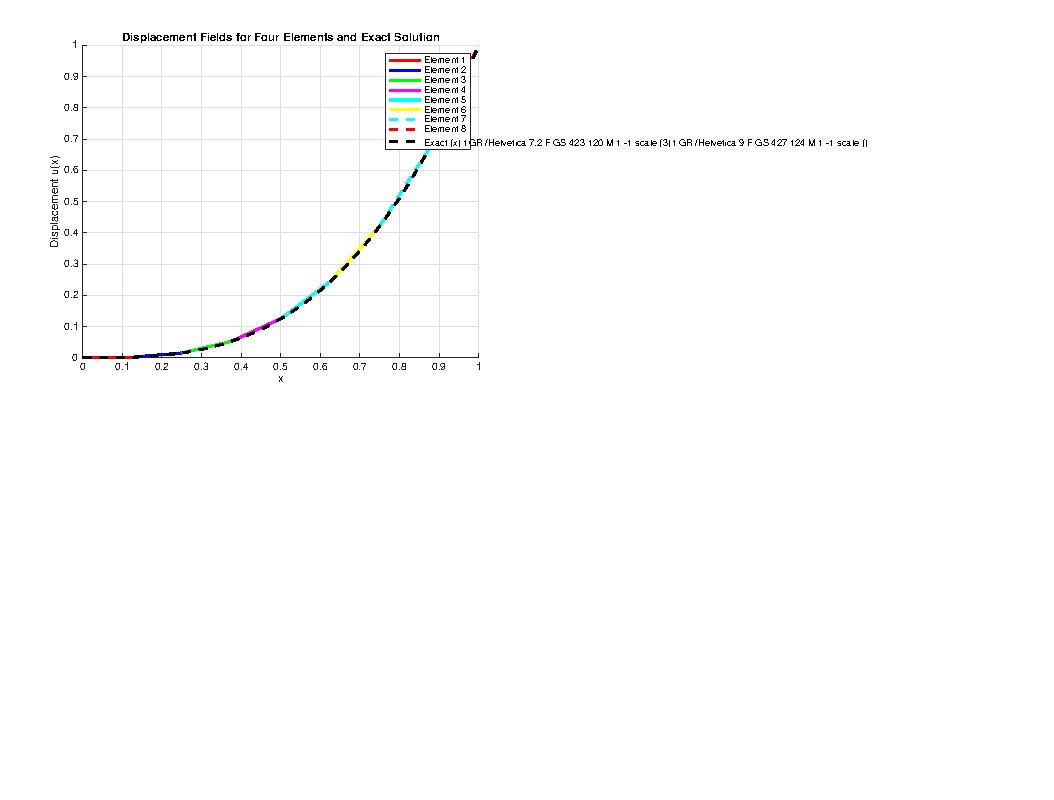
\includegraphics[width=\maxwidth{56.196688409433015em}]{figure_6.eps}
\end{center}

\begin{par}
\begin{flushleft}
			
\end{flushleft}
\end{par}

\begin{matlabcode}
% Compute B^e for all elements
B_1 = 8*[-1 1];
B_2 = 8*[-1 1];
B_3 = 8*[-1 1];
B_4 = 8*[-1 1];
B_5 = 8*[-1 1];
B_6 = 8*[-1 1];
B_7 = 8*[-1 1];
B_8 = 8*[-1 1];

% Set up a matrix for the displacement vector
d_1 = [u_11 ; u_12];
d_2 = [u_21 ; u_22];
d_3 = [u_31 ; u_32];
d_4 = [u_41 ; u_42];
d_5 = [u_51 ; u_52];
d_6 = [u_61 ; u_62];
d_7 = [u_71 ; u_72];
d_8 = [u_81 ; u_82];

% Strain displacement for element 1 and element 2

e_1 = B_1 * d_1;
e_2 = B_2 * d_2;
e_3 = B_3 * d_3;
e_4 = B_4 * d_4;
e_5 = B_5 * d_5;
e_6 = B_6 * d_6;
e_7 = B_7 * d_7;
e_8 = B_8 * d_8;

% Display computed strains for all elements
disp(e_1);
\end{matlabcode}
\begin{matlaboutput}
   0.015625000000000
\end{matlaboutput}
\begin{matlabcode}
disp(e_2);
\end{matlabcode}
\begin{matlaboutput}
   0.109375000000000
\end{matlaboutput}
\begin{matlabcode}
disp(e_3);
\end{matlabcode}
\begin{matlaboutput}
   0.296875000000000
\end{matlaboutput}
\begin{matlabcode}
disp(e_4);
\end{matlabcode}
\begin{matlaboutput}
   0.578125000000000
\end{matlaboutput}
\begin{matlabcode}
disp(e_5);
\end{matlabcode}
\begin{matlaboutput}
   0.953125000000000
\end{matlaboutput}
\begin{matlabcode}
disp(e_6);
\end{matlabcode}
\begin{matlaboutput}
   1.421875000000000
\end{matlaboutput}
\begin{matlabcode}
disp(e_7);
\end{matlabcode}
\begin{matlaboutput}
   1.984375000000000
\end{matlaboutput}
\begin{matlabcode}
disp(e_8);
\end{matlabcode}
\begin{matlaboutput}
   2.640625000000000
\end{matlaboutput}
\begin{matlabcode}

% Define the range of x values for each element (renaming to avoid overwriting previous variables)
x_vals_strain_element1 = linspace(x1, x2, 100);  % For Element 1
x_vals_strain_element2 = linspace(x2, x3, 100);  % For Element 2
x_vals_strain_element3 = linspace(x3, x4, 100);  % For Element 3
x_vals_strain_element4 = linspace(x4, x5, 100);  % For Element 4
x_vals_strain_element5 = linspace(x5, x6, 100);  % For Element 5
x_vals_strain_element6 = linspace(x6, x7, 100);  % For Element 6
x_vals_strain_element7 = linspace(x7, x8, 100);  % For Element 7
x_vals_strain_element8 = linspace(x8, x9, 100);  % For Element 8
x_vals_exact_strain = linspace(x1, x9, 200);     % For the exact solution over the whole domain

% Define the strain for each element (constant within each element)
strain_element1 = e_1(1);  % Strain in element 1
strain_element2 = e_2(1);  % Strain in element 2
strain_element3 = e_3(1);  % Strain in element 3
strain_element4 = e_4(1);  % Strain in element 4
strain_element5 = e_5(1);  % Strain in element 5
strain_element6 = e_6(1);  % Strain in element 6
strain_element7 = e_7(1);  % Strain in element 7
strain_element8 = e_8(1);  % Strain in element 8

% Plot the strain fields
figure;
hold on;  % Allow multiple plots on the same figure

% Plot Element 1 strain (constant)
plot(x_vals_strain_element1, strain_element1 * ones(size(x_vals_strain_element1)), 'r', 'LineWidth', 2, 'DisplayName', 'Element 1 Strain');
% Plot Element 2 strain (constant)
plot(x_vals_strain_element2, strain_element2 * ones(size(x_vals_strain_element2)), 'b', 'LineWidth', 2, 'DisplayName', 'Element 2 Strain');
% Plot Element 3 strain (constant)
plot(x_vals_strain_element3, strain_element3 * ones(size(x_vals_strain_element3)), 'g', 'LineWidth', 2, 'DisplayName', 'Element 3 Strain');
% Plot Element 4 strain (constant)
plot(x_vals_strain_element4, strain_element4 * ones(size(x_vals_strain_element4)), 'm', 'LineWidth', 2, 'DisplayName', 'Element 4 Strain');
% Plot Element 5 strain (constant)
plot(x_vals_strain_element5, strain_element5 * ones(size(x_vals_strain_element5)), 'c', 'LineWidth', 2, 'DisplayName', 'Element 5 Strain');
% Plot Element 6 strain (constant)
plot(x_vals_strain_element6, strain_element6 * ones(size(x_vals_strain_element6)), 'y', 'LineWidth', 2, 'DisplayName', 'Element 6 Strain');
% Plot Element 7 strain (constant)
plot(x_vals_strain_element7, strain_element7 * ones(size(x_vals_strain_element7)), 'c--', 'LineWidth', 2, 'DisplayName', 'Element 7 Strain');
% Plot Element 8 strain (constant)
plot(x_vals_strain_element8, strain_element8 * ones(size(x_vals_strain_element8)), 'r--', 'LineWidth', 2, 'DisplayName', 'Element 8 Strain');
% Plot the exact strain
exact_strain = 3 * x_vals_exact_strain.^2;
plot(x_vals_exact_strain, exact_strain, 'k--', 'LineWidth', 2, 'DisplayName', 'Exact Strain (3x^2)');

% Add labels and title
xlabel('x');
ylabel('Strain \epsilon(x)');
title('Finite Element Strain vs Exact Strain');
legend show;  % Show legend
grid on;
hold off;
\end{matlabcode}
\begin{center}
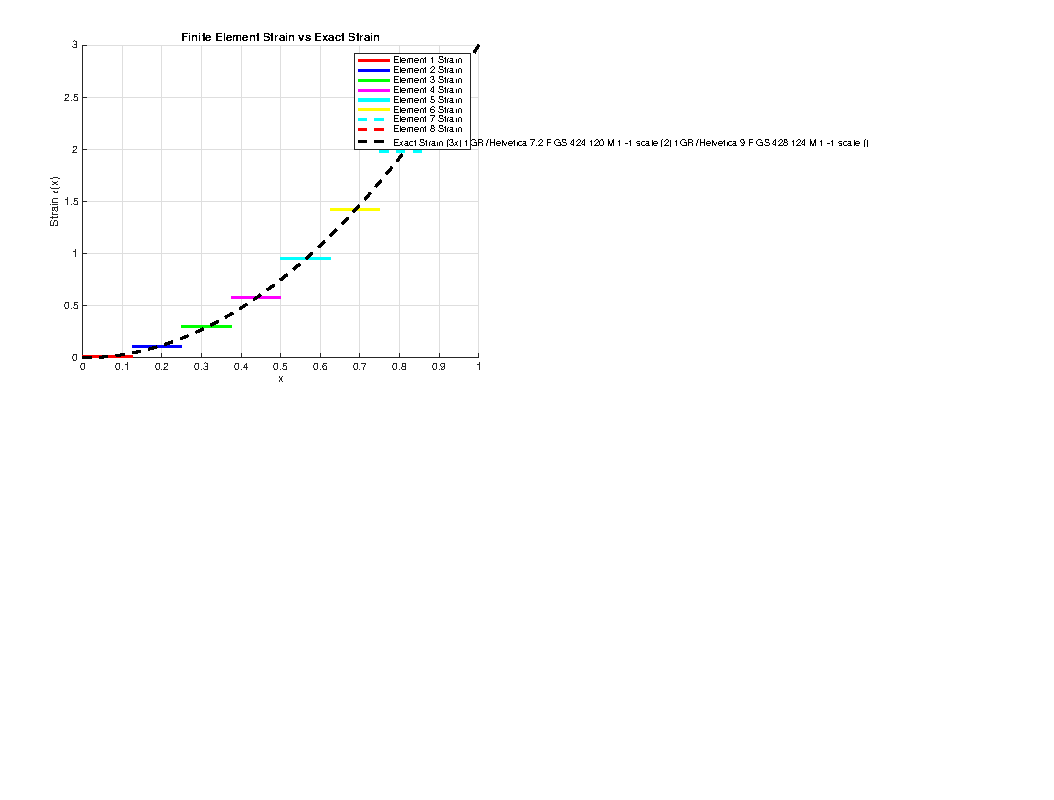
\includegraphics[width=\maxwidth{56.196688409433015em}]{figure_7.eps}
\end{center}

\begin{par}
\begin{flushleft}
As we increase the elements, we get a better fit for the displacement field. Eight elements follows the actual displacement field equation fairly well. As for the strain, we are still getting constant values, but they trend with the displacement field. So the more elements we use, the mroe accurate the results.
\end{flushleft}
\end{par}


\vspace{1em}
\matlabheadingthree{Part D:}

\matlabheadingthree{The error of an interpolation is generally measured by what is called a L2 norm. The error in the L2 norm, which we denote by e, is given by $e=\int_0^L (u^e -u)^2 \,dx$ where $~u=x^3$ in this case. Compute the error e for meshes of two, four and eight linear displacement elements. Use Gauss quadrature for integration. Then plot (this can be done manually) the error versus the element size on a log-log plot. This should almost be a straight line. What is its slope? This slope is indicative of the rate of convergence of the element.}


\vspace{1em}
\begin{matlabcode}
% Define the exact solution u(x) = x^3 as an anonymous function
% @(x): This defines an anonymous function where x is the input variable.
% x.^3: This is the function body, which means the output of the function is
% x^3 . The .^ operator ensures that this works element-wise (in case x is a vector or matrix).
exact_solution = @(x) x.^3;

% Define the Gauss quadrature points and weights for a 2-point rule
% These were given in the Table in chapter 4
gauss_points = [-sqrt(1/3), sqrt(1/3)];  % Gauss points in [-1, 1]
gauss_weights = [1, 1];  % Weights for 2-point quadrature

% Initialize an array (3x1 matrix) to store the L2 norm error for 2, 4, and 8 elements
error_L2 = zeros(3, 1);  % To store errors for each mesh size

% Define the mesh sizes
mesh_sizes = [2, 4, 8];
L = 1;  % Length of the domain is 1 from part a

% Loop over each mesh size so that it will run the values for 2, 4, and 8
% elements.
for mesh_index = 1:length(mesh_sizes)
    num_elements = mesh_sizes(mesh_index);  % Get the number of elements
    element_length = L / num_elements;  % Compute the length of each element
    error_sum = 0;  % Initialize the error sum for this mesh size
    
    % Loop over each element
    for elem = 1:num_elements
        % Define element boundaries for each element
        x1 = (elem - 1) * element_length;  % Left node of element
        x2 = elem * element_length;        % Right node of element
        
        % linear shape function for the element
        u_h = @(x) ((x2 - x) / element_length) * exact_solution(x1) + ...
                   ((x - x1) / element_length) * exact_solution(x2);
        
        % Compute the squared error for each Gauss point
        for i = 1:length(gauss_points)
            % Map Gauss point to the actual element
            xi = ((x2 - x1) / 2) * gauss_points(i) + (x2 + x1) / 2;
            
            % Compute the error at the Gauss point
            error_at_gauss_point = (u_h(xi) - exact_solution(xi))^2;
            
            % Sum the contribution of this Gauss point
            error_sum = error_sum + gauss_weights(i) * error_at_gauss_point * (x2 - x1) / 2;
        end
    end
    
    % Store the L2 norm error for this mesh size
    error_L2(mesh_index) = sqrt(error_sum);
end

% Plot the error vs element size (log-log plot)
element_sizes = 1 ./ mesh_sizes;  % Element size = 1 / number of elements
figure;
loglog(element_sizes, error_L2, '-o', 'LineWidth', 2);
xlabel('Element Size (h)');
ylabel('L2 Norm of Error');
title('L2 Norm Error vs Element Size');
grid on;
\end{matlabcode}
\begin{center}
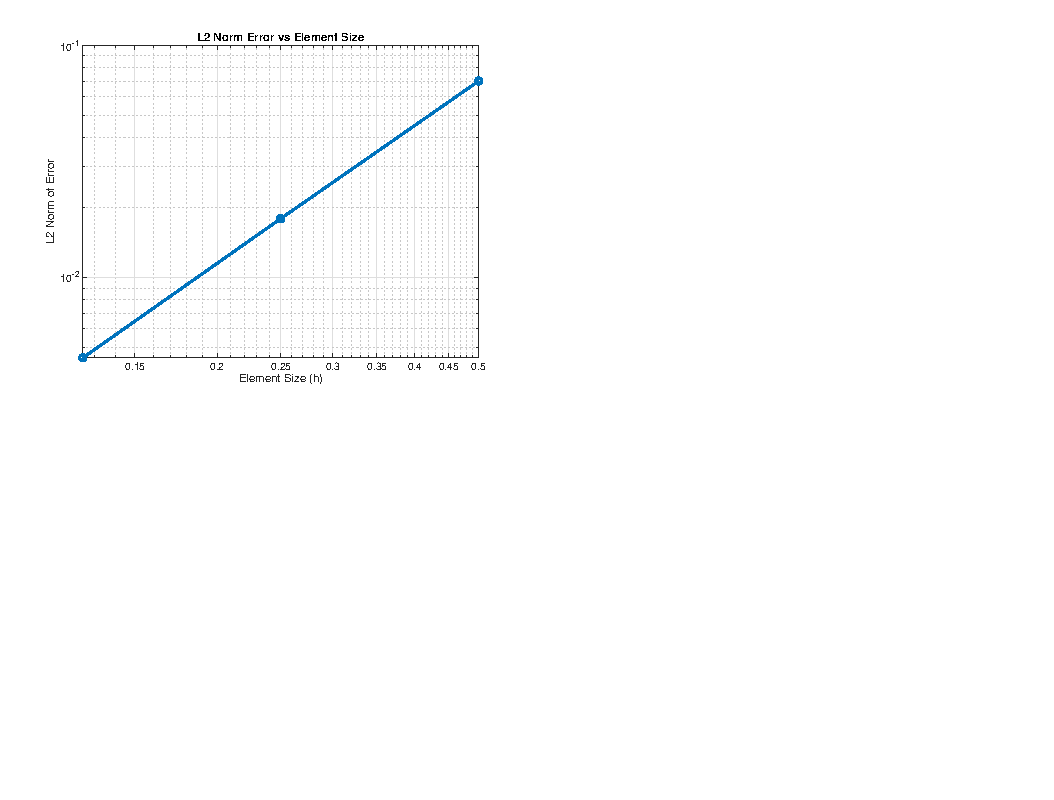
\includegraphics[width=\maxwidth{56.196688409433015em}]{figure_8.eps}
\end{center}
\begin{matlabcode}

% Optionally, compute the slope of the log-log plot (convergence rate)
p = polyfit(log(element_sizes), log(error_L2), 1);
fprintf('Slope of the log-log plot (rate of convergence): %.2f\n', p(1));
\end{matlabcode}
\begin{matlaboutput}
Slope of the log-log plot (rate of convergence): 1.98
\end{matlaboutput}

\matlabheadingthree{Part E:}

\matlabheadingthree{Repeat part (d) using quadratic two-node quadratic elements. 						}

\begin{par}
\hfill \break
\end{par}

\begin{matlabcode}
% Define the exact solution u(x) = x^3 as an anonymous function
exact_solution = @(x) x.^3;

% Define the Gauss quadrature points and weights for a 3-point rule (since we are now using quadratic elements)
gauss_points = [-sqrt(3/5), 0, sqrt(3/5)];  % Gauss points in [-1, 1]
gauss_weights = [5/9, 8/9, 5/9];  % Weights for 3-point quadrature

% Initialize an array to store the L2 norm error for 2, 4, and 8 elements
error_L2 = zeros(3, 1);  % To store errors for each mesh size

% Define the mesh sizes
mesh_sizes = [2, 4, 8];
L = 1;  % Length of the domain

% Loop over each mesh size
for mesh_index = 1:length(mesh_sizes)
    num_elements = mesh_sizes(mesh_index);  % Get the number of elements
    element_length = L / num_elements;  % Compute the length of each element
    error_sum = 0;  % Initialize the error sum for this mesh size
    
    % Loop over each element
    for elem = 1:num_elements
        % Define element boundaries and mid-point
        x1 = (elem - 1) * element_length;  % Left node of element
        x3 = elem * element_length;        % Right node of element
        x2 = (x1 + x3) / 2;               % Mid-point of element
        
        % Finite element approximation for this element (quadratic shape functions)
        N1 = @(x) (x - x2) * (x - x3) / ((x1 - x2) * (x1 - x3));
        N2 = @(x) (x - x1) * (x - x3) / ((x2 - x1) * (x2 - x3));
        N3 = @(x) (x - x1) * (x - x2) / ((x3 - x1) * (x3 - x2));
        
        % Approximate displacement u^e for the element using the shape functions
        u_h = @(x) N1(x) * exact_solution(x1) + N2(x) * exact_solution(x2) + N3(x) * exact_solution(x3);
        
        % Compute the squared error for each Gauss point
        for i = 1:length(gauss_points)
            % Map Gauss point to the actual element
            xi = ((x3 - x1) / 2) * gauss_points(i) + (x3 + x1) / 2;
            
            % Compute the error at the Gauss point
            error_at_gauss_point = (u_h(xi) - exact_solution(xi))^2;
            
            % Sum the contribution of this Gauss point
            error_sum = error_sum + gauss_weights(i) * error_at_gauss_point * (x3 - x1) / 2;
        end
    end
    
    % Store the L2 norm error for this mesh size
    error_L2(mesh_index) = sqrt(error_sum);
end

% Plot the error vs element size (log-log plot)
element_sizes = 1 ./ mesh_sizes;  % Element size = 1 / number of elements
figure;
loglog(element_sizes, error_L2, '-o', 'LineWidth', 2);
xlabel('Element Size (h)');
ylabel('L2 Norm of Error');
title('L2 Norm Error vs Element Size (Quadratic Elements)');
grid on;
\end{matlabcode}
\begin{center}
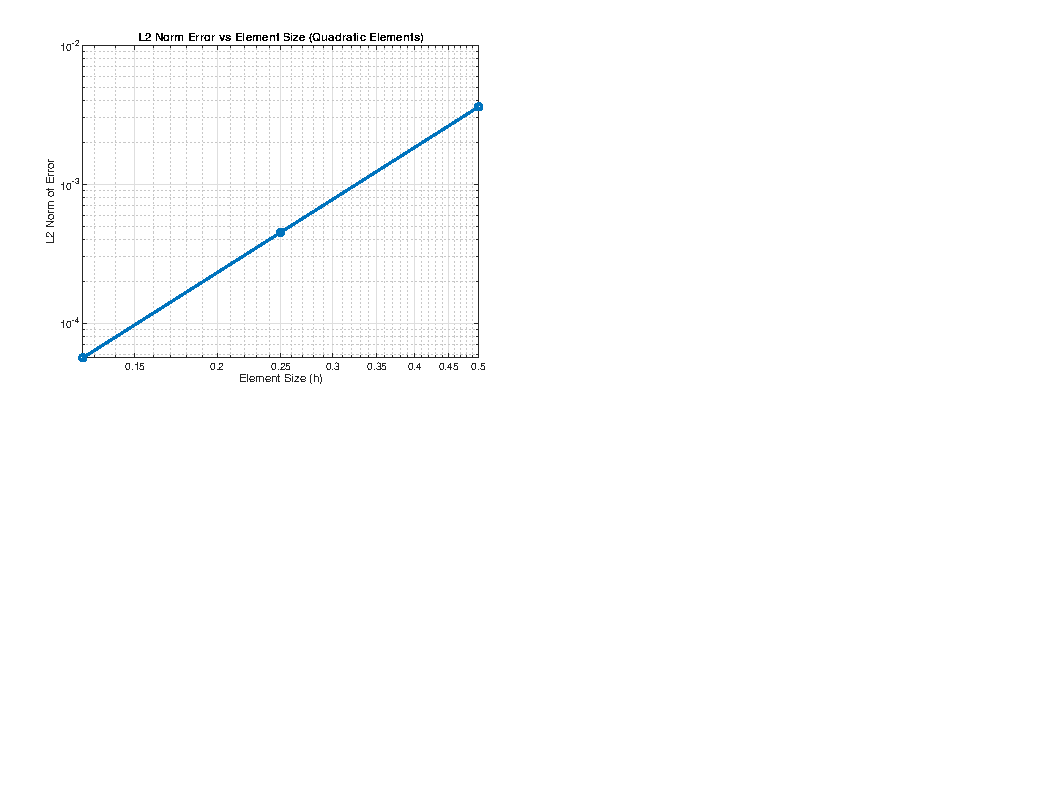
\includegraphics[width=\maxwidth{56.196688409433015em}]{figure_9.eps}
\end{center}
\begin{matlabcode}

% Optionally, compute the slope of the log-log plot (convergence rate)
p = polyfit(log(element_sizes), log(error_L2), 1);
fprintf('Slope of the log-log plot (rate of convergence for quadratic elements): %.2f\n', p(1));
\end{matlabcode}
\begin{matlaboutput}
Slope of the log-log plot (rate of convergence for quadratic elements): 3.00
\end{matlaboutput}


\begin{par}
\begin{flushleft}
				
\end{flushleft}
\end{par}

\matlabheadingtwo{Problem 4.6}

\matlabheadingtwo{Use Gauss quadrature to obtain exact values for the following integrals. Verify by analytical integration: }


\vspace{1em}
\matlabheadingthree{a.) $\int_0^4 (x^2 +1)\,dx$}

\begin{par}
\hfill \break
\end{par}

\begin{matlabcode}
% Define the function to integrate f(x) = x^2 + 1
f = @(x) x.^2 + 1;

% Define the Gauss points and weights for the interval [-1, 1]
gauss_points = [-sqrt(1/3), sqrt(1/3)];
gauss_weights = [1, 1];

% Define the transformation from [-1, 1] to [0, 4]
a = 0;
b = 4;
transformation = @(xi) (b - a) / 2 * xi + (b + a) / 2;
jacobian = (b - a) / 2;

% Compute the Gauss quadrature approximation
integral_gauss = 0;
for i = 1:length(gauss_points)
    xi = gauss_points(i);
    integral_gauss = integral_gauss + gauss_weights(i) * f(transformation(xi)) * jacobian;
end

% Display the result
fprintf('Gauss quadrature approximation of integral from 0 to 4 of (x^2 + 1) dx: %.6f\n', integral_gauss);
\end{matlabcode}
\begin{matlaboutput}
Gauss quadrature approximation of integral from 0 to 4 of (x^2 + 1) dx: 25.333333
\end{matlaboutput}
\begin{matlabcode}

% Compute the analytical solution
analytical_solution = integral(@(x) x.^2 + 1, 0, 4);
fprintf('Analytical solution: %.6f\n', analytical_solution);
\end{matlabcode}
\begin{matlaboutput}
Analytical solution: 25.333333
\end{matlaboutput}
\begin{matlabcode}

\end{matlabcode}

\matlabheadingthree{b.) $\int_{-1}^1 (\xi^4 +2\xi^2 )\,dx$}

\begin{par}
\hfill \break
\end{par}

\begin{matlabcode}
% Define the function to integrate f(xi) = xi^4 + 2xi^2
f = @(xi) xi.^4 + 2*xi.^2;

% Gauss quadrature for [-1, 1] (already in the interval)
integral_gauss = 0;
for i = 1:length(gauss_points)
    xi = gauss_points(i);
    integral_gauss = integral_gauss + gauss_weights(i) * f(xi);
end

% Display the result
fprintf('Gauss quadrature approximation of integral from -1 to 1 of (xi^4 + 2xi^2) dxi: %.6f\n', integral_gauss);
\end{matlabcode}
\begin{matlaboutput}
Gauss quadrature approximation of integral from -1 to 1 of (xi^4 + 2xi^2) dxi: 1.555556
\end{matlaboutput}
\begin{matlabcode}

% Compute the analytical solution
analytical_solution = integral(@(xi) xi.^4 + 2*xi.^2, -1, 1);
fprintf('Analytical solution: %.6f\n', analytical_solution);
\end{matlabcode}
\begin{matlaboutput}
Analytical solution: 1.733333
\end{matlaboutput}

\begin{par}
\begin{flushleft}
				
\end{flushleft}
\end{par}

\begin{par}
\begin{flushleft}
			
\end{flushleft}
\end{par}

\begin{par}
\begin{flushleft}
		
\end{flushleft}
\end{par}

\begin{par}
\begin{flushleft}
	 
\end{flushleft}
\end{par}

\begin{par}
\begin{flushleft}
		
\end{flushleft}
\end{par}

\begin{par}
\begin{flushleft}
					
\end{flushleft}
\end{par}

\begin{par}
\begin{flushleft}
				
\end{flushleft}
\end{par}

\begin{par}
\begin{flushleft}
			
\end{flushleft}
\end{par}

\begin{par}
\begin{flushleft}
		
\end{flushleft}
\end{par}

\begin{par}
\begin{flushleft}
	 
\end{flushleft}
\end{par}


\vspace{1em}
\begin{par}
\begin{flushleft}
	 
\end{flushleft}
\end{par}

\end{document}
